% 原图的点、曲线、刻度与图例数值不变，只叠加中文文字。
\begin{tikzpicture}
\node[anchor=south west,inner sep=0] (plot) at (0,0) {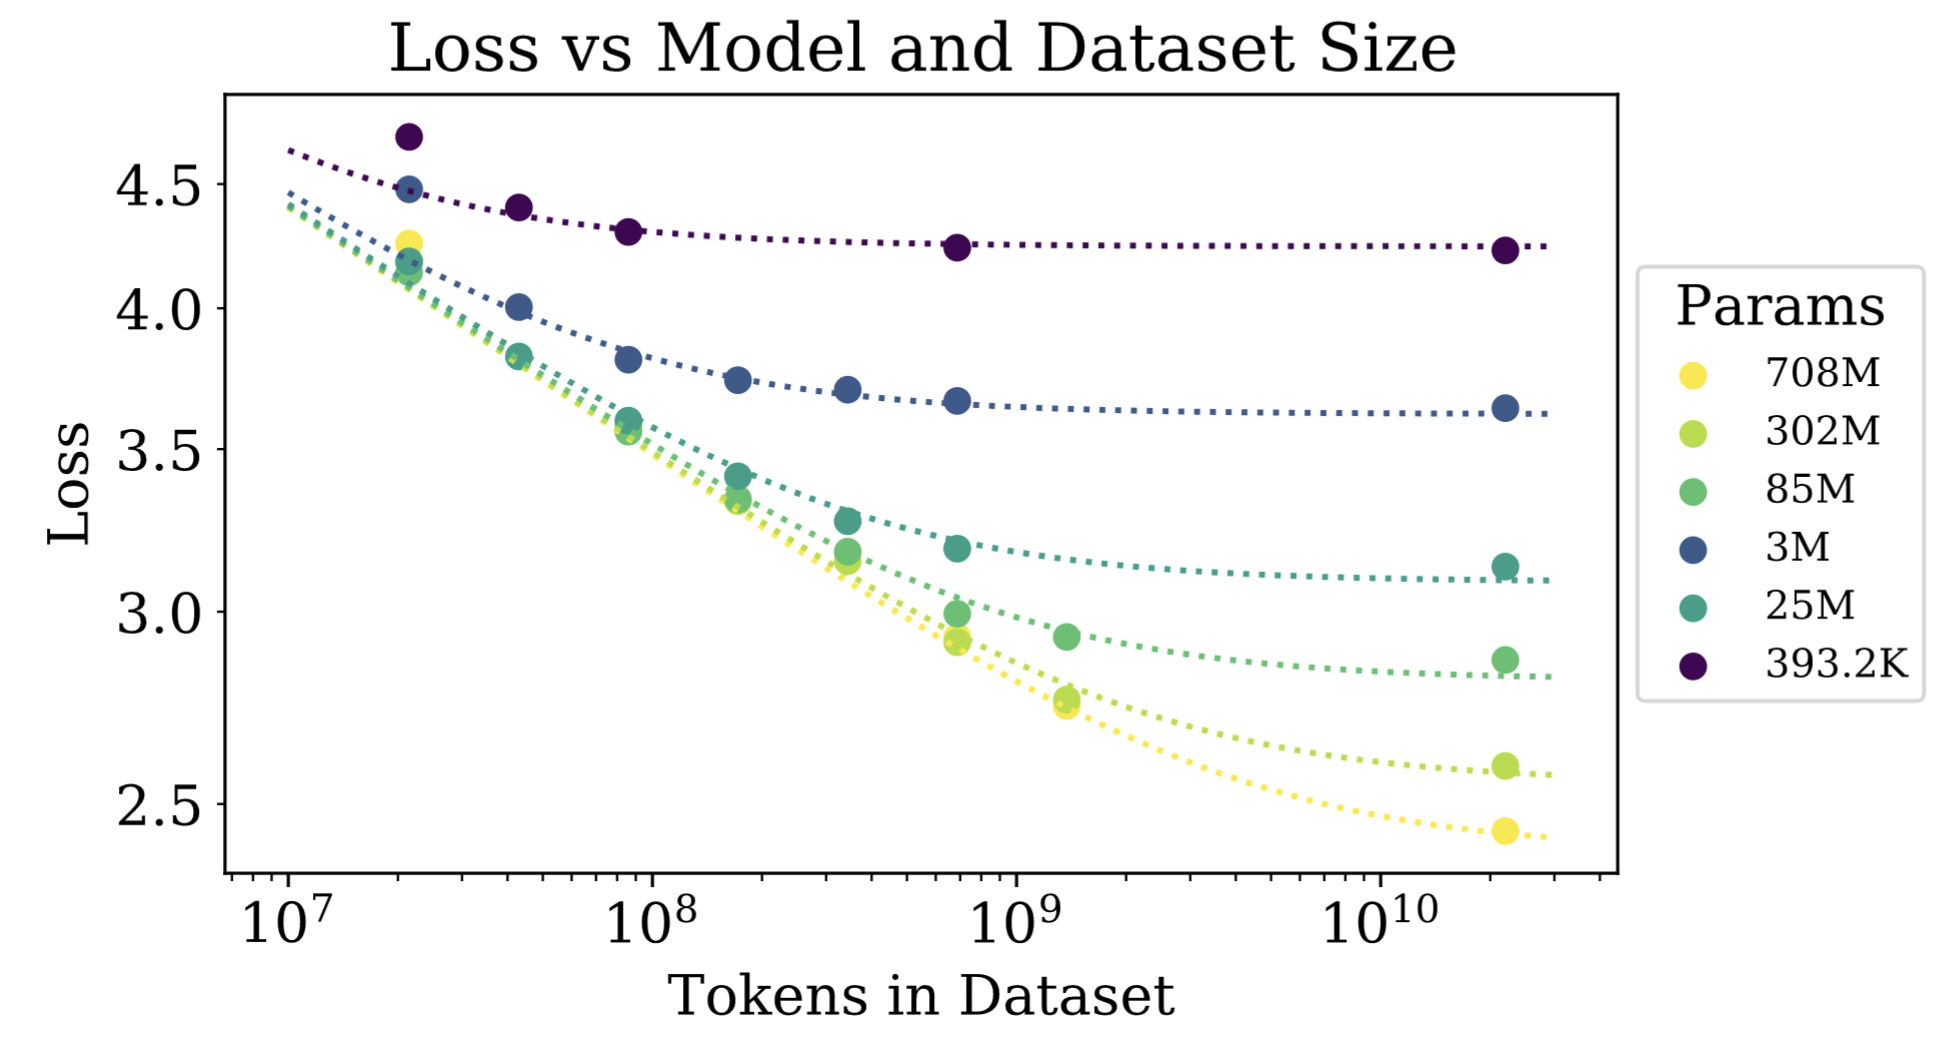
\includegraphics[width=.7\linewidth]{part1/visuals/sample_efficiency_tokens.png}};
\begin{scope}[x={(plot.south east)},y={(plot.north west)},every node/.style={font=\scriptsize,inner sep=0pt}]
\fill[white] (.15,.915) rectangle (.85,1);
\node[font=\small] at (.5,.965) {损失与模型规模、数据集规模的关系};
\fill[white] (0,.40) rectangle (.05,.75);
\node[rotate=90] at (.026,.55) {损失};
\fill[white] (.30,0) rectangle (.77,.092);
\node at (.53,.035) {数据集中的词元数};
\fill[white] (.845,.685) rectangle (.99,.755);
\node at (.918,.72) {参数量};
\end{scope}
\end{tikzpicture}
